\section{External Source}\label{sec:external_source}
An alternative method of context enrichment is based on fetching concept definitions from external sources, especially when these are not already available as metadata annotations in the ontologies that are validated. The lookup is solely based on the concept's name, neglecting the connected nature of an ontology. Dictionaries have always been the first choice when it comes to searching for specific information about words or phrases.

This section begins with an introduction in the theory of dictionaries, discusses searching problems and strategies to overcome these and briefly describes several online dictionaries including the one we used in our approach.

\paragraph{Short Introduction into Lexicography}
Dictionaries, as most humans are familiar with, contain the \textit{lexicon} of a language, that is a collection of words or phrases, called the lexemes. 
They are designed for word lookups and facilitate finding information about spelling, meaning and usage. Historically, written dictionaries were constrained by the alphabetised format and once printed, never updated. On the other hand, online dictionaries facilitate accessing the information on more than one path, semantics being one of them. Similarly, keeping the word up-to-date as well as adding new ones is as simple as updating or adding new records to the database, compared to printing and distributing new copies of their written pedants. 

Lexicography is defined as the science about~\enquote{the theory and practice of dictionaries, that is, dictionaries, encyclopaedias, lexica, glossaries, vocabularies, terminological knowledge bases, and other information tools covering areas of knowledge and its corresponding language.}~\cite{fuertes2017}
Among other definitions, they share the understanding that lexicography is an interdisciplinary science with characteristics of linguistic science, information science and others. 

When it comes to classifying electronic dictionaries, it is obvious that they are more than just machine-readable copies of their printed counterparts, but rather comprehensive software conglomerates only limited by technological, economical and/or practical constraints. The key defining elements of electronic dictionaries are 
\begin{inparaenum}[i)]
		\item the access principle,
		\item the construction principle and
		\item the distinction between information databases and information tools
\end{inparaenum}~\cite{fuertes2011}.
Whereas the \textit{access principle} deals with providing quick and easy access to the needed information, the \textit{construction principle} differentiates dictionaries based on the technical and economical aspects when building the dictionary. Special attention should be paid to the division between information databases and information tools, that is, separating user concerns~(searching and viewing the results) from the underlying data organisation. 

Depending on the usage scenarios, several types of dictionaries have emerged over the years. A recent study~\cite{mueller_spitzer2013} evaluated, how dictionaries are being used or, in other words, the external conditions or situations in which a dictionary consultation is embedded.  
In their research, participants with professional and academic background were asked about the circumstances of dictionary usage. 
Analyses revealed that responses can be partitioned into the following \textit{groups of usage} situations: 
\begin{enumerate}
	\item Text Production
	\item Text Reception
	\item Text Translation
\end{enumerate}

\textit{Text Production} is the action of writing texts in professional or personal contexts. Dictionary content vary in many ways, depending on writer's profession and text category. For example, passive speech using domain specific vocabularies are dominant in academic literature over active speech and simple language constructs in short-term, informal texts~\cite{o2010routledge}~(e.g. emails, tweets, Facebook posts, \ldots).

\textit{Text Reception} is the process or theory that emphasises the meaning and interpretation of existing literature. Readers focus on writing reviews and understanding texts. The user's motivation of dictionary interaction is finding the word definition as well as looking for samples~(e.g. example sentences), synonyms/antonyms and links to external information. 

\textit{Text Translation} is the process of converting text from a source language to a target language by preserving its meaning. Unfortunately there is not always a one-to-one mapping possible because of lacking equivalent language constructs in the target language. Old-fashioned dictionaries containing translations for specific words do not help either because words are lacking context. With the advent of online dictionaries, new opportunities for translators appeared such as spelling correction and links to synonyms/antonyms. Not only professional translators responded that dictionaries are crucial for their business, students and teachers consult dictionaries to improve their vocabulary, look up pronunciation or simply find the contexts of word usage. 

\paragraph{Searching in Electronic Dictionaries} Searching is probably the most important feature of today's electronic dictionaries. In the next paragraphs we discuss problems that arise when searching for specific terms and strategies to overcome these. 

Several studies~\cite{pastor2010, mvechura2008} have analysed digital dictionaries, available in different languages and accessible via the Internet or compressed on a digital medium~(e.g. CD-ROM). Their evaluation is based on empirical analyses of user behaviour collected from log-files as well as literature review. All searching techniques listed below tackle the problem of invalid, incomplete, misspelled and multi-word search queries.

The first category are \textit{inflection-aware} search algorithms which accept inflected and uninflected search queries. The central part of these algorithms are rewrite rules which transform the input query to the matching headword or vice-versa. A powerful but complicated technique is based on a deep understanding of the target language. It is based on morphologies of the word endings. For example, stripping \emph{-ed} and \emph{-ing} endings for regular verbs is yet simple but only manageable for regular verbs, more complicated algorithms are needed for irregular verbs. Other algorithms, not taking the structure of the target language into account, are based on fuzzy string searching, a technique based on approximate string matching. A simple metric measuring the difference between two strings is the Levenshtein~Distance~\cite{levenshtein1966}. It is defined as the number of single character manipulations necessary to transform one string into the other. 

The next category are algorithms dealing with \textit{multi-word} search items. Search algorithms need to deal with user entered search strings, containing multiple words or even complete sentences. The situation is even more complicated, for a single-word search query users expect not only matching single-word entries but also matching multi-word entries~(e.g. phrasal verb). Enumerating all possible word combinations might be acceptable in dictionaries with small corpora, but it is infeasible in dictionaries with millions of entries and performance is important. In these cases it is better to construct an index from single-word entries and multi-word entries. An even better approach, also known by the term \emph{lemmatising}, would be to analyse and process the words before-hand.

Another challenge in processing search queries is \textit{detecting misspellings}. User input is inherently prone to errors. Smart algorithms guide the user to the intended word by offering corrections and suggestions, similar to what a spellchecker does. A naive approach would be to collect lists of common misspelled words and continue with matching. This has the disadvantage that not all possible combinations are included and processing takes longer, especially for long word lists. A better but yet more complicated technique is based on word similarity which is discussed in the previous paragraph. 

A technique especially useful for multi-lingual dictionaries is \textit{language selection and detection}. As there already exists much literature in this area~\cite{mcnamee2005, lodhi2002, vatanen2010, selamat2016}, we decided to just outline two approaches here. The first group of algorithms is purely based on statistical models. The detection of the target language works by building probabilistic models of the inferred statistics and the pre-trained statistics. The second group works by counting common words or character sequences~(called n-grams) and comparing the obtained frequency counts against reference values~\cite{mcnamee2005}.

The last technique is \textit{text normalisation}. It solves the problem of unwanted characters in search strings by removing variation and reducing words to simpler formats. For search strings, this means that noisy characters are removed. A simple strategy is to delete characters which do not add any meaning such as hyphens, dots quotation marks and (mathematical)~symbols. Additionally, consecutive occurrences of whitespaces are merged. 
The normaliser also need to consider some character variations as defined by the Unicode~Standard\footnote{\url{http://www.unicode.org/reports/tr15/} accessed 2018/06/08 }. 

\paragraph{Online Dictionary Examples} We have chosen some well-known, freely accessible online dictionaries that were used in various research
fields.

%WordNet
Started as a research project in 1985 at Princeton University \textbf{WordNet}~\cite{fellbaum1998} is best characterised as a dictionary browser rather than just an online dictionary. It allows users to explore its contents on the basis of semantic, rather than alphabetic similarities. Users look up information along more than one path, semantics being among them. How one wants to explore the possibilities of online dictionaries rather depends on one's ideas and applications one has in mind. 

The building blocks of WordNet are \textit{synsets} which are defined as sets of words having similar semantics~(synonymy). It is important that synonymy does not entail unrestricted interchangeability. By that criterion natural languages would have very few synonyms. Instead, synonymy is typically relative to a context which is encoded as links between and within synsets. 
Several linguistic relations are defined in WordNet, for example \textit{polysemy/monosemy}, \textit{hyponymy/hypernymy} and \textit{meronymy/holonymy}. 
Polysemy/Monosemy describes the fact that a word may have multiple meanings or one meaning. Hyponymy/Hypernymy means that words or phrases are included in the meaning of another word. Meronymy/Holonymy describes part-of or member-of relationships.

The WordNet architecture~\cite{fellbaum1998} as illustrated in~\hyperref[fig:wordnet_architecture]{Figure~\ref*{fig:wordnet_architecture}} can be split into these parts:
\begin{enumerate}
		\item Lexical Source Files
		\item the Grinder
		\item the Lexical Database
		\item Software Tools and Interfaces
\end{enumerate}

\begin{figure}
	 \centering
	 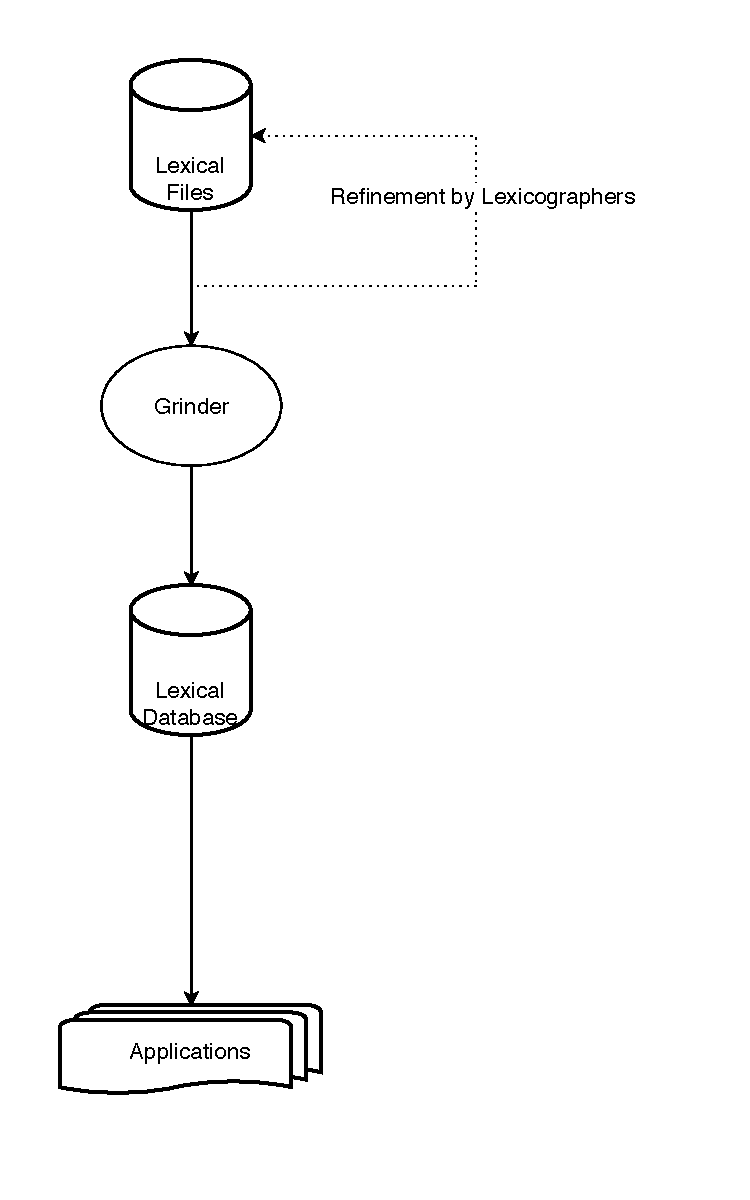
\includegraphics[width=0.5\textwidth]{drawio/WordNet_Architecture}
	 \caption{The architecture of the WordNet System~\cite{fellbaum1998}}\label{fig:wordnet_architecture}
\end{figure}


The \textit{Lexical Database} forms the heart of the WordNet system. It is the result of processing all lexical source files. There are many tools available, written in various programming languages like Perl or awk, to interact with the database. 

WordNet offers some \textit{interfaces} to users for interaction. Depending on the area of application there are textual interfaces~(Command Line Interfaces and APIs) and graphical interfaces~(Desktop Software and Web Applications). Invoking the search form and starting search tasks can also be done via browser interface\footnote{\url{http://wordnetweb.princeton.edu/perl/webwn} accessed 2018/06/14}.

WordNet's key success factor is its potentials in terms of Natural Language Processing~(NLP). It was also used as information source in many other fields~\cite{morato2004}, these are: Image Retrieval, Information Retrieval, Document Classification, Query Expansion, Machine Translation and Conceptual Disambiguation.

A different approach was taken by \textbf{WordNik}\footnote{\url{https://www.wordnik.com/} accessed 2018/06/15}. It targets native English speakers who look up words that are rare~(technical terms or dialect terms), very old or very new. They often search for definitional information which is incomplete or missing in traditional dictionaries. Users tolerate published imperfection because they opt for relevant, actual and cutting-edge information, even though not officially approved by editors~\cite{burnett1979}. They want to understand the context of word usage in sentences, not necessarily explanatory statements as in printed or even online dictionaries.

The driving force behind WordNik was contribution. It processes and aggregates external user-generated content such as tweets, newspaper articles, scientific articles or uploaded Flickr\footnote{\url{https://www.flickr.com/} accessed 2018/06/15} images. This is similar to what search engines do, but with restricted scope. The creators of WordNik observed that very few people write word definitions, they rather add meta linguistic information such as lists of their favourite words, comments or tags. WordNik additionally collects statistics about lexicographical terms, more or less frequently searched words and most commented words. 

WordNik also offers an API for programmatically accessing their resources\footnote{\url{https://developer.wordnik.com/} accessed 2018/06/15}. At the time of writing this thesis free access is granted for non-profit, non-commercial use with a limitation on the number of API calls. 
After a successful registration process, an API token is provided which is a prerequisite for API interaction. Besides Web access, a handful of libraries\footnote{\url{https://developer.wordnik.com/libraries} accessed 2018/06/15}, available in many programming languages, were created to facilitate integration with third-party applications. 

\textbf{Wiktionary}\footnote{\url{https://www.wiktionary.org/} accessed 2018/06/15} is a freely accessible, collaborative online lexicon~\cite{granger2012}. Whereas traditional dictionaries are the product of a small group of expert lexicographers, collaboratively constructed dictionaries are created by many, not necessarily expert users. This has the advantage that new lexical entries are added more frequently and existing ones are continuously updated. Users are encouraged to participate in content creation and maintenance. New lexical entries are discussed in the community until a consensus is reached. 

An important goal of Wiktionary is openness towards multilingualism. It was first launched in 2002 and indented as an "add-on" to Wikipedia\footnote{\url{https://www.wikipedia.org/} accessed 2018/06/16}. At that time it was only available in English, but now translations exist for nearly every spoken language. However, they differ in scope and community size. Each Wiktionary is accessible by prepending the respective ISO~639~language~code\footnote{\url{https://www.iso.org/iso-639-language-codes.html} accessed 2018/06/16} to the common wiktionary domain.

Content is organised as collections of pages, each containing a title and a body. There are four page categories:
\begin{inparaenum}[1)]
		\item Article Pages,
		\item Redirect Pages,
		\item Talk Pages and
		\item Internal Pages
\end{inparaenum}.
Most pages are \emph{Article Pages}, containing the actual linguistic information. With \emph{Redirect Pages}, users are able to navigate from page to page. At page creation, \emph{Talk Pages} help editors in collecting ideas, expressing criticism, asking questions and discussing page contents. \emph{Internal Pages} are protected and contain motivational information, goals, statistics, indices, appendices and guidelines for contributors. 

Wiktionary is not targeted to specific groups of people nor its content serves a specific purpose, instead, it is open for everyone. 
Linguistic knowledge is organised in separate sections as explained in the next paragraphs: 

It may sound surprising that each page starts with the \emph{language} of the term or phrase because each page belongs to a specific translation of Wiktionary anyway. However, this is necessary because the same term can be encoded in multiple languages. For example, the term \texttt{boat} is used in five languages\footnote{\url{https://en.wiktionary.org/wiki/boat} accessed 2018/06/16}. 

The \textit{etymology} section describes origin and history of a word. It helps linguists in exploring linguistic relations such as synonymy/antonymy, hypernymy/hyponymy and homonymy/polysemy. They are also interested, whether and how the meaning has changed over time. 

\textit{Phonetic references} are appreciated not only by language learners but also by readers who are unfamiliar with particular terms. The term's pronunciation is encoded using audio samples or phonetic notations. 

In contrast to other dictionaries which focus on canonical word forms, Wiktionary also contains entries for inflected word forms. For example, the English verb \texttt{go} and its \textit{morphology} \texttt{went} are encoded as separate entries. Additionally, it may include the declension of an adjective or the conjunction of a verb.

Each term is associated with a \textit{syntactic category} which includes part of speech tags for single words, idioms, proverbs and multi-word expressions. Apart from these, there are also other tags available. For example, nouns are marked as countable/uncountable or singular/plural. 

The most interesting part for dictionary readers is probably the section \textit{semantic knowledge} which describes the meaning of a term. It includes example sentences, quotations, links to other terms, glosses and linguistic labels. The gloss of a word is either a marginal or interlinear notation of the word's meaning. Non-linguists are eventually more familiar with the term \emph{glossary} which denotes to collections of glosses. 

\textit{Cross-lingual knowledge} is especially important for translators and educators who are interested in multilingual realtions. This is expressed as links between pages of differing language. For example, descriptions of the English word \texttt{boat} are contained in a page with links to \texttt{water~craft}, \texttt{full-house} and conformation to \texttt{cyclohexane}.

A valuable feature for non-native speakers is \emph{graphical knowledge}. It is obvious that humans grasp the meaning of a term faster by just looking at a picture or photograph than reading through long textual descriptions. Unfortunately, not all terms can be expressed in pictures or photographs though. 

From a technical perspective Wiktionary is based on MediaWiki\footnote{\url{https://www.mediawiki.org/wiki/MediaWiki} accessed 2018/06/17}, a free and open source software written in PHP\footnote{\url{http://www.php.net/} accessed 2018/06/17}. The software is distributed under the GNU~General~Public~License~(GPL) and maintained by the WikiMedia~Foundation\footnote{\url{https://wikimediafoundation.org/wiki/Home} accessed 2018/06/17}, a non-profit organisation aimed at supporting free, multilingual, educational content. MediaWiki is also used by many other wikis\footnote{\url{https://wikistats.wmflabs.org/} accessed 2018/06/17}.

The majority of wiki features are accessible via public API. Clients can request features or send commands over the \textit{MediaWiki~Action~API}\footnote{\url{https://www.mediawiki.org/wiki/API:Main_page} accessed 2018/06/17}. It has querying, searching, parsing and manipulation capabilities.

\paragraph{Dictionary based Approach}\label{sec:enrichment_dictionary_approach}
Intuitively, the idea of generating descriptions using dictionary lookups is simple: starting from a concept name, descriptions are built from consulting an online dictionary. 

A schematic overview of the overall workflow is shown in~\hyperref[fig:external_source_workflow]{Figure~\ref*{fig:external_source_workflow}}.
\begin{figure}
	 \centering
	 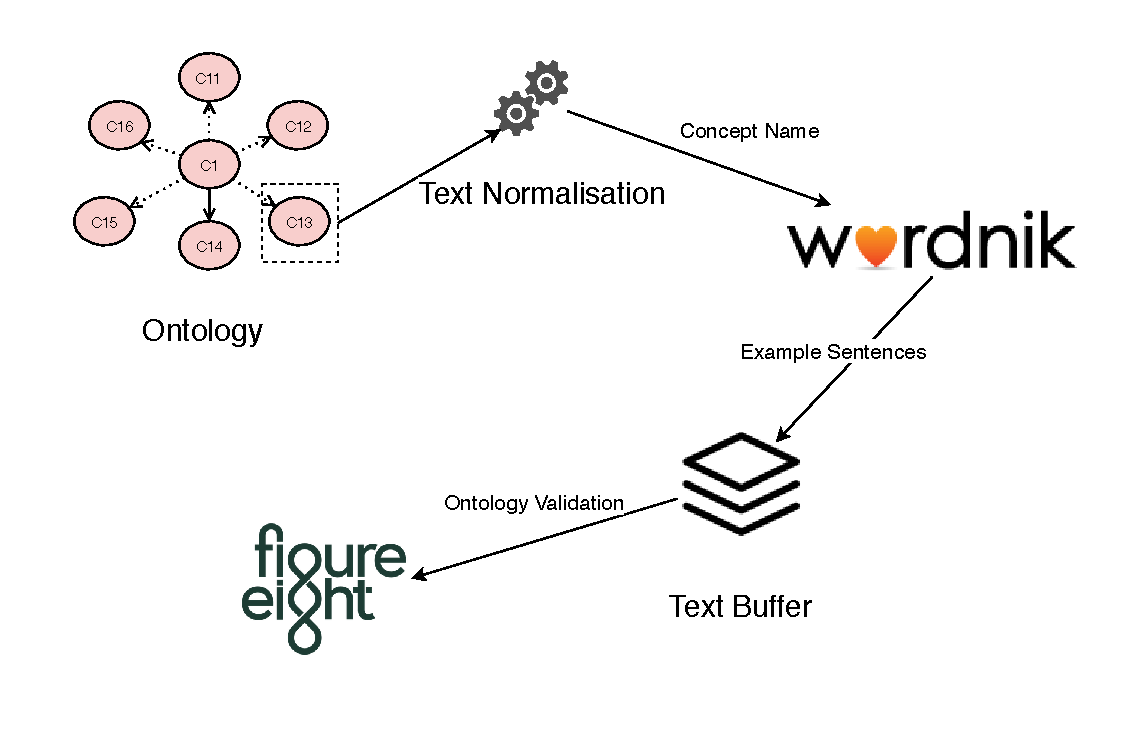
\includegraphics[width=0.9\textwidth]{drawio/External_Source_Workflow}
	 \caption{Conceptual workflow of WordNik consultation to generate concept descriptions}\label{fig:external_source_workflow}
\end{figure}
The idea is to use the concept name as a baseline for any further processing. Often, the name can not be used directly as input to WordNik because it contains unwanted characters such as excessive spaces, quotes, dots or just non-printable characters. This is especially true for learned ontologies, generated from textual sources. Our algorithm uses the built-in text manipulation capabilities of the JDK to pre-process concept names. Among the other approaches introduced earlier in this section, it is yet simple but still provides good results. 

Next, WordNik is consulted to find example sentences for normalised concept names. In contrast to traditional dictionaries, WordNik searches in all kinds of available online content, including newspapers, journals, scientific publications, tweets and others. 
All API interaction is protected against unauthorised access, however, to help developers learning the API, some features are available in isolated Sandbox~Mode\footnote{\url{https://developer.wordnik.com/docs} accessed  2018/06/21}. For instance, example sentences for the word \texttt{bird} can be fetched from the URL \texttt{/word.json/bird/examples}.

Depending on wether a single concept or multiple concepts are validated, example sentences need to be harmonised, which is realised by storing intermediate results and mapping these to the initial concepts. 

To conclude, this approach is rather simple and easy to implement, however, it may have the potential to generate wrong results, especially for ambiguous concept names. 
